\section{Methodology Descripttion}
\subsection{Data Collection}
\subsubsection{Data Sources}
Para el proceso de extraccion de datos, se utilizo las resenas y especificaciones de productos de la pagina \href{https://pricebaba.com/}{pricebaba}. Esta pagina web proporciona una amplia gama de productos, incluidos telefonos moviles, laptops, televisores, y otros dispositivos electronicos. Para esta investigacion, inicialmente se utilizara unicamente los datos de los telefonos mobiles. La pagina brinda informacion detallada de los productos, junto con las resenas de los personas expertas; por ello, es una fuente valiosa de datos para entrenar y evaluar los modelos de generacion de resenas.
\\\\
Las resenas tienen una estructura como la imagen \ref{fig:pricebaba-review-structure}, donde se puede observar que cada resena contiene descripcion detallada del producto, pros y contras, y descripcion del producto enfocada a diferentes caracteristicas como camara, bateria, pantalla, etc. Ademas en la imagen \ref{fig:pricebaba-spec-structure} se puede observar que las especificaciones del producto estan estructuradas en forma de tabla y subtablas, lo cual facilita la extraccion de datos.
\begin{figure}[H]
    \centering
    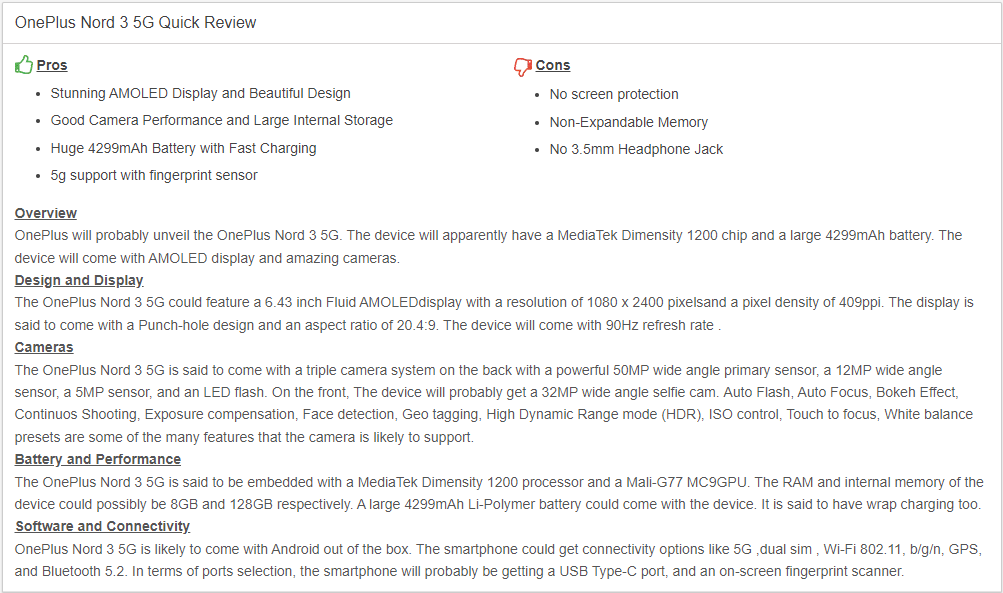
\includegraphics[width=12cm]{images/pricebaba_review_structure.png}
    \caption{pricebaba reviews structure}
    \label{fig:pricebaba-review-structure}
\end{figure}
\begin{figure}[H]
    \centering
    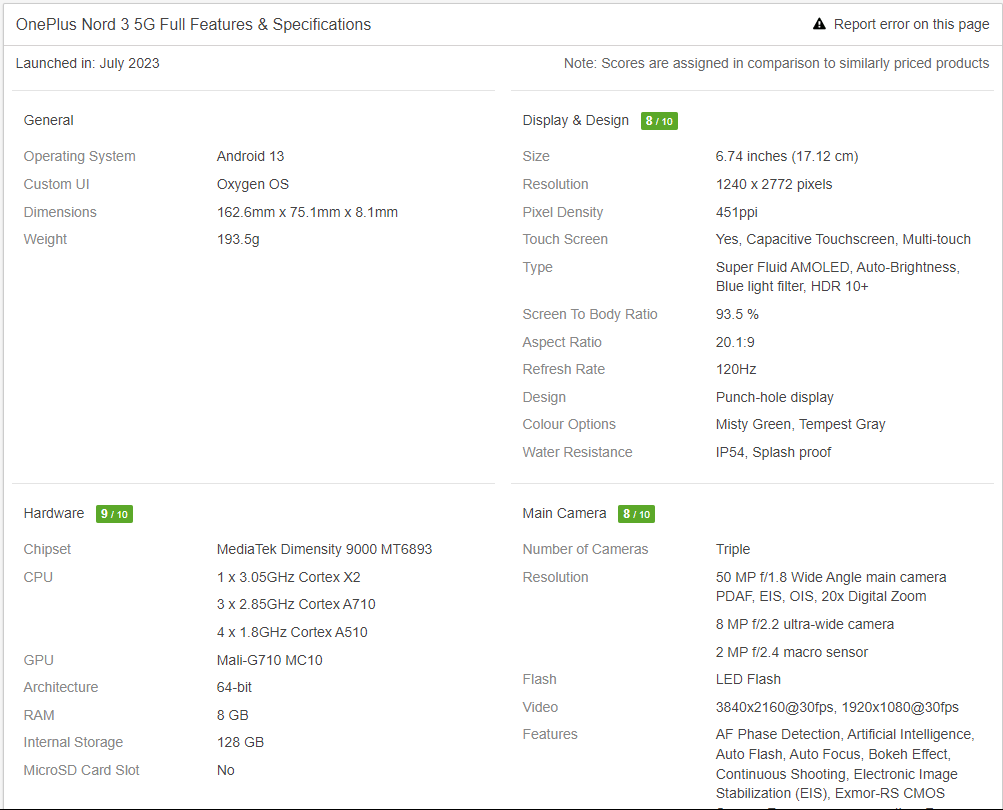
\includegraphics[width=12cm]{images/pricebaba_spec_structure.png}
    \caption{pricebaba specifications structure}
    \label{fig:pricebaba-spec-structure}
\end{figure}
Para lograr la extraccion de datos, se utilizara la tecnica de \textit{web scraping}, que consiste en extraer informacion de paginas web y almacenarla en una base de datos. En este caso, se extraeran las resenas y especificaciones de los telefonos moviles de pricebaba y se almacenaran en formato JSON para su posterior procesamiento. De esta manera se logro obtener un \textit{dataset} de resenas y otro de especificaciones de 7400 telefonos moviles que servira como base de datos inicial para su limpieza y formateo.

\subsubsection{Data Format}
El formato escogido para la representacion de los datos es JSON, con este formato se logra representar los datos de manera estructurada y facil de procesar. Se utilizara dos JSONs para representar los datos, uno para las resenas y otro para las especificaciones de los productos. Cada JSON contendra un arreglo de objetos, donde cada objeto representara un producto con sus respectivas resenas o especificaciones. La estructura de los JSONs se muestra a continuacion:
\newpage
\begin{lstlisting}[style=jsonstyle, frame = single, caption=JSON Data Format Product specification, label=code:json-data-format]
    {
        "url": {
            "Launch Date": "Launch Date",
            "General": {
                "subcategories1": [
                    "value1"
                    ],
                "subcategories2": [
                    "value1",
                    "value2"
                    ],
                ...
            },
            "Characteristic1": {
                "subcategories1": [
                    "value1"
                    ],
                "subcategories2": [
                    "value1",
                    "value2"
                    ],
                ...
            },
            "Characteristic2": {
                "subcategories1": [
                    "value1"
                    ],
                "subcategories2": [
                    "value1",
                    "value2"
                    ],
                ...
            },
            ...
        },
    }
\end{lstlisting}
\newpage
\begin{lstlisting}[style=jsonstyle, frame = single, caption=JSON Data Format reviews, label=code:json-data-format]
    {
        "url": {
            "text": {
                "Characteristic1": ["Description1"],
                "Characteristic2": ["Description2"],
                ...
            },
            "Pros": [
                "Pro 1",
                "Pro 2",
                "Pro 3"
            ],
            "Cons": [
                "Con 1",
                "Con 2",
                "Con 3"
            ]
        },
    }
    \end{lstlisting}

\subsubsection{Data Cleaning Process}
Una vez que se han extraido los datos, es necesario realizar un proceso de limpieza para garantizar que los datos sean coherentes y esten listos para ser procesados por los modelos. Por ello se realizaran las siguientes tareas de limpieza:


\subsubsection{Normalization} 
Una vez que ya se tienen los datos estructurados en JSON, se procede a normalizarlos. Para esto se evaluo las llaves de los objetos y se limpiaron las llaves con espacios en blanco, se transformaron las llaves, subllaves y valores a minusculas, se cambiaron los \& por `and' y se reordenaron las llaves que incluyeran `and' para que tengan un orden logico. Por ejemplo, la llave `Display \& Design' se cambio a `Design and Display'.

\subsubsection{Data Removal} 
Una vez que toda la data esta normalizada, se procede a eliminar duplicados y datos que se consideran no necesarios. Para esto se eliminaran las resenas que no contengan ningun valor en la llave `text', las especificaciones que solo contengan el valor `General' o las resenas que solo contengan el valor `Overview'. Esto debido a que buscamos realizar resenas de productos de acuerdo a sus diferentes caracteristicas de manera detallada y no de manera general.

\subsubsection{Split data}
Una vez que se han limpiado y estructurado los datos, se procede a dividir el dataset en tres conjuntos: entrenamiento, y prueba. Para esto se utilizara una proporcion de 80\% para entrenamiento y 20\% para prueba. De esta manera se garantiza que los modelos se entrenen con una cantidad suficiente de datos y se evaluen de manera adecuada. 
\\\\
Se priorizo utilizar los datos de los productos mas recientes para el conjunto de prueba, para que los modelos sean evaluados con datos mas actuales evitando asi que el modelo encuentre datos similares dentro de su corte de entrenamiento. Para esto, se ordeno el \textit{dataset} por la llave `Launch Date' de manera descendente y se seleccionaron los primeros 20\% de los datos para el conjunto de prueba. De esta manera se garantiza que los modelos sean evaluados con datos mas recientes y se evita que los modelos memoricen los datos de entrenamiento.

\subsubsection{Prompt structuration}
Cuando ya se han limpiado los JSONs de resenas y especificaciones, se procede a estructurar las instrucciones que se utilizaran para entrenar los modelos. Estas instrucciones formaran el dataset final. Para esto se crearan instrucciones de la siguiente estructura:
\begin{lstlisting}[style=textstyle, frame = single, caption=Prompt structuration, label=code:prompt-structuration]
"Given following json that contains specifications of a product, generate a review of the key characteristics with json format. Follow the structure on Keys to write the Output: 
### Product: Product for JSON specifications
### Keys: Combination of the keys of the JSON reviews
### Output: reviews for JSON reviews accordingly to the keys"
\end{lstlisting}
Cuando se hace refeerencia a las permutaciones en \ref{code:prompt-structuration} se refiere a que se generaran instrucciones para cada permutacion de las llaves de las resenas. Por ejemplo, si se tiene una resena con las llaves `Design and Display', `Camera', `Battery', `Performance', `Software', se escogen `i' instrucciones de las posibles combinaciones de las llaves, donde `i' es el numero de instrucciones que se desean generar. De esta manera se logra que el modelo genere resenas de acuerdo a las diferentes caracteristicas de los productos. Un ejemplo de selccion de llaves seria que si se tiene un producto con las llaves `Design and Display', `Camera', `Battery', `Performance', `Software', se seleccionen las llaves `Design and Display', `Camera' para generar una instruccion, para otra instruccion para el mismo producto se seleccionen las llaves `Design and Display', `Battery', y asi sucesivamente.
\\\\
Con estas combinaciones de llaves para la generacion de instrucciones se obtienen de los 7400 datos originales, 60700 instrucciones que se utilizaran para entrenar los modelos. Estas instrucciones son el dataset final el cual se encuentra en \href{https://huggingface.co/datasets/kokujin/json_data_luis}{Hugginface}.

\subsection{Model Fine-Tuning}
\subsubsection{Hyperparameter Selection}
Debido a que los LLMs que se van a utilizar ya son modelos preentrenados, los hiperparametros que se van a seleccionar son los que se utilizan para el proceso de afinacion de los modelos. 
Ademas, por limitaciones de computo se seleccionaran los hiperparametros que se ajusten a las capacidades de la maquina en la que se va a realizar el proceso de afinacion. Para esto se seleccionaran los hiperparametros de la tabla \ref{table:hyperparameters}.
\begin{table}[H]
    \centering
    \begin{tabular}{|c|c|}
        \hline
        \textbf{Hyperparameter} & \textbf{Value} \\
        \hline
        Learning Rate & 2e-4 \\
        Batch Size & 2 \\
        Epochs & 1 \\
        max\_grad\_norm & 0.3 \\
        gradient\_accumulation\_steps & 1 \\
        weight\_decay & 0.001 \\
        warmup\_ratio & 0.03 \\
        lr\_scheduler\_type & cosine \\
        optim & adam \\
        max\_seq\_length & 900 \\
        \hline
    \end{tabular}
    \caption{Hyperparameters Selection}
    \label{table:hyperparameters}
\end{table}
The choose of the `max\_seq\_length' is because before it estimate the average token length of the reviews and it was 900 tokens. To do that it was necessary to iterate every prompt and tokenizer. Ademas, se ha utilizado la libreria de `BitsAndBytesConfig' de `transformers' de Hugginface para la optimizacion del modelo. Estos hiperparametros adicionales son los que se muestran en la tabla \ref{table:hyperparameters-bitsandbytes}.
\begin{table}[H]
    \centering
    \begin{tabular}{|c|c|}
        \hline
        \textbf{Hyperparameter} & \textbf{Value} \\
        \hline
        bnb\_4bit\_compute\_dtype & float16 \\
        bnb\_4bit\_quant\_type & nf4 \\
        use\_nested\_quant & False \\
        \hline
    \end{tabular}
    \caption{Hyperparameters Selection BitsAndBytes}
    \label{table:hyperparameters-bitsandbytes}
\end{table}

\subsection{Model Evaluation}
Una vez que los modelos han sido afinados, se procede a evaluarlos con los datos de prueba. Para esto se utilizaron las metricas de BLEU, METEOR y ROUGE. Estas metricas se utilizan comparando las resenas generadas por los modelos con las resenas reales de los productos. De esta manera se logra evaluar la calidad de las resenas generadas por los modelos y se determina cual es el modelo que mejor se ajusta a los datos de prueba.